%%%%%%%%%%%%%%%%%%%%%%%%%%%%%%%%%%%%%
%                                   %
% Compile with XeLaTeX and biber    %
%                                   %
% Questions or comments:            %
%                                   %
% joshua dot mcneill at uga dot edu %
%                                   %
%%%%%%%%%%%%%%%%%%%%%%%%%%%%%%%%%%%%%

\documentclass{beamer}
  % Read in standard preamble (cosmetic stuff)
  %%%%%%%%%%%%%%%%%%%%%%%%%%%%%%%%%%%%%%%%%%%%%%%%%%%%%%%%%%%%%%%%
% This is a standard preamble used in for all slide documents. %
% It basically contains cosmetic settings.                     %
%                                                              %
% Joshua McNeill                                               %
% joshua dot mcneill at uga dot edu                            %
%%%%%%%%%%%%%%%%%%%%%%%%%%%%%%%%%%%%%%%%%%%%%%%%%%%%%%%%%%%%%%%%

% Beamer settings
% \usetheme{Berkeley}
\usetheme{CambridgeUS}
% \usecolortheme{dove}
% \usecolortheme{rose}
\usecolortheme{seagull}
\usefonttheme{professionalfonts}
\usefonttheme{serif}
\setbeamertemplate{bibliography item}{}

% Packages and settings
\usepackage{fontspec}
  \setmainfont{Charis SIL}
\usepackage{hyperref}
  \hypersetup{colorlinks=true,
              allcolors=blue}
\usepackage{graphicx}
  \graphicspath{{../../figures/}}
\usepackage[normalem]{ulem}
\usepackage{enumerate}

% Document information
\author{M. McNeill}
\title[FREN2001]{Français 2001}
\institute{\url{joshua.mcneill@uga.edu}}
\date{}

%% Custom commands
% Lexical items
\newcommand{\lexi}[1]{\textit{#1}}
% Gloss
\newcommand{\gloss}[1]{`#1'}
\newcommand{\tinygloss}[1]{{\tiny`#1'}}
% Orthographic representations
\newcommand{\orth}[1]{$\langle$#1$\rangle$}
% Utterances (pragmatics)
\newcommand{\uttr}[1]{`#1'}
% Sentences (pragmatics)
\newcommand{\sent}[1]{\textit{#1}}
% Base dir for definitions
\newcommand{\defs}{../definitions}


  % Packages and settings

  % Document information
  \subtitle[Révision, examen 1]{Révision pour l'examen 1}

\begin{document}
  % Read in the standard intro slides (title page and table of contents)
  \begin{frame}
    \titlepage
    \tiny{Office: % Basically a variable for office hours location
Gilbert 121\\
          Office hours: % Basically a variable for office hours
 lundi, mercredi, vendredi 10:10--11:10
}
  \end{frame}

  \begin{frame}{}
    \hypertarget{début}{}
    \begin{columns}
      \column{0.5\textwidth}
        \begin{center}
          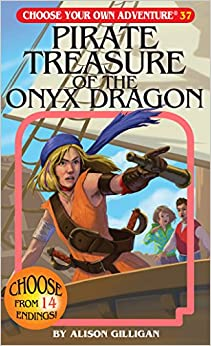
\includegraphics[scale=0.3]{aventure.jpg} \\
          Le Trésor de pirate du dragon d'onyx
        \end{center}
      \column{0.5\textwidth}
        Tu es sur un bâteau.
        Tu sens ...
        \begin{enumerate}
          \item \hyperlink{questions}{des questions} au nord.
          \item \hyperlink{passé}{le passé} à l'est.
          \item \hyperlink{pronoms}{des pronoms} au sud.
          \item \hyperlink{modes}{des modes} à l'ouest.
        \end{enumerate}
        Choisis une direction.
    \end{columns}
  \end{frame}

  \begin{frame}{Questions}
    \hypertarget{questions}{}
    \begin{columns}
      \column{0.5\textwidth}
        Tu trouves un vaisseau fantôme dans un orage.
        Tu décide de poser des questions au capitaine.
        Tu peux utiliser ...
        \begin{enumerate}
          \item les mots \hyperlink{que}{\lexi{qui} et \lexi{que}}.
          \item le mot \hyperlink{quel}{\lexi{quel/le/s}}.
        \end{enumerate}
        Ou tu peux retourner \hyperlink{début}{au sud} si tu as peur...
      \column{0.5\textwidth}
        \begin{center}
          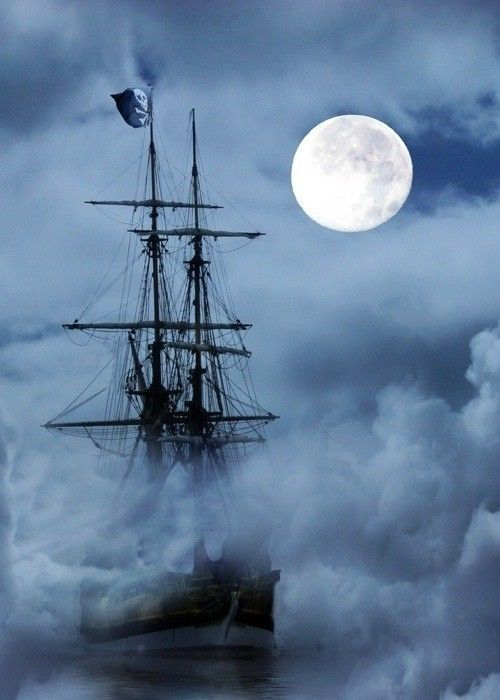
\includegraphics[scale=0.5]{vaisseau.jpg}
        \end{center}
    \end{columns}
  \end{frame}

  \begin{frame}{Passé}
    \hypertarget{passé}{}
    \begin{columns}
      \column{0.5\textwidth}
        Tu te trouves sur une île inhabitée.
        Dans le sable, tu vois des leçons de grammaire.
        Tu peux examiner ...
        \begin{enumerate}
          \item \hyperlink{composé}{le passé composé}.
          \item \hyperlink{imparfait}{l'imparfait}.
        \end{enumerate}
        Si tu as de la chance, tu peux construire un canoë et retourner \hyperlink{mort}{à l'ouest}...
      \column{0.5\textwidth}
        \begin{center}
          \includegraphics[scale=0.5\textwidth]{inhabitée.jpg}
        \end{center}
    \end{columns}
  \end{frame}

  \begin{frame}{}
    \hypertarget{pronoms}{Pronoms}
    \begin{columns}
      \column{0.5\textwidth}
        Il y a un monstre de mer.
        Tu le vois, et tu réféchis à l'attaquer.
        Tu peux l'attaquer avec ...
        \begin{enumerate}
          \item \hyperlink{direct}{des objets directs}.
          \item \hyperlink{indirect}{des objets indirects}.
          \item \hyperlink{y}{le pronom \lexi{y}}.
        \end{enumerate}
        Ou tu peux retourner \hyperlink{début}{au nord} si tu as peur...
      \column{0.5\textwidth}
        \begin{center}
          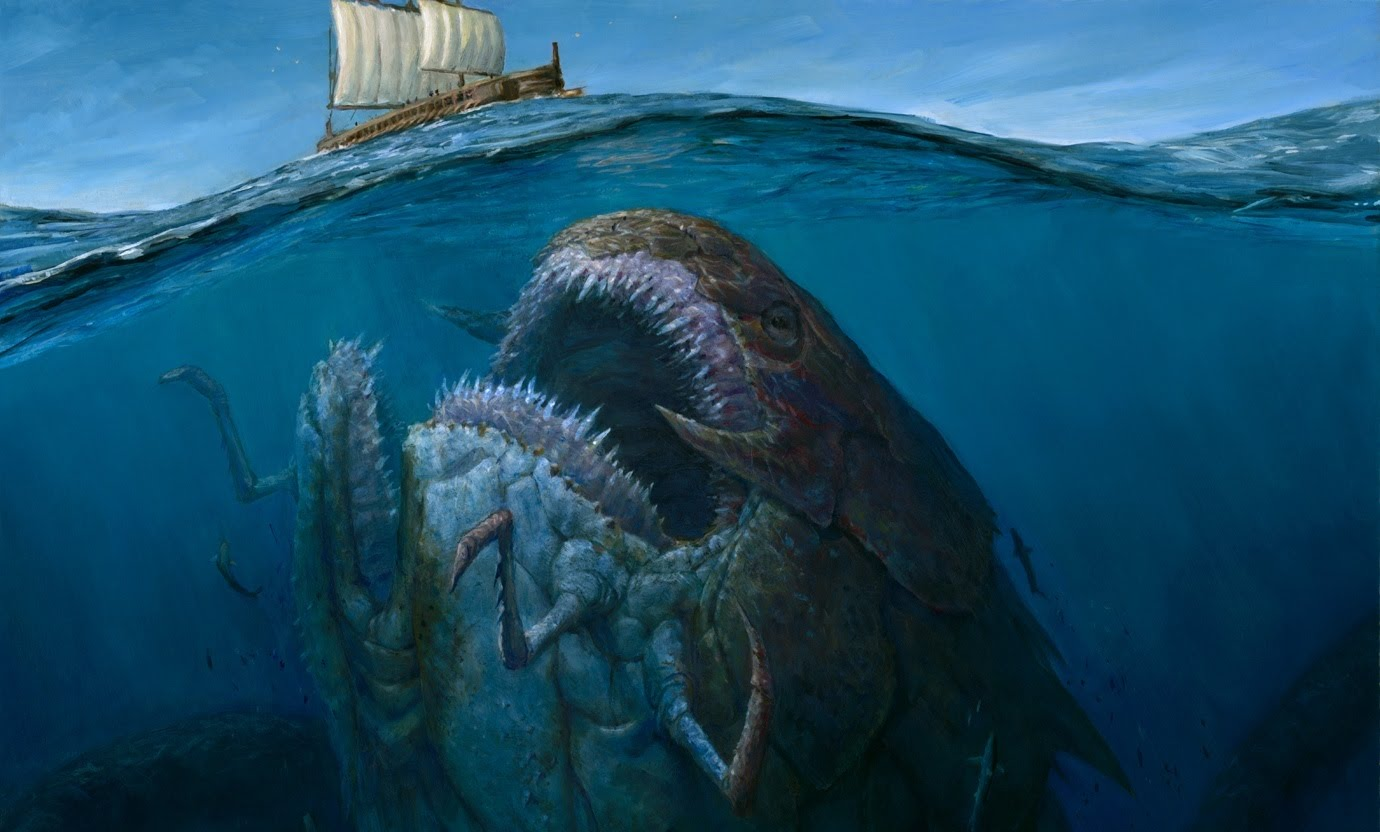
\includegraphics[scale=0.5]{monstre.jpg}
        \end{center}
    \end{columns}
  \end{frame}

  \begin{frame}{Modes}
    \hypertarget{modes}{}
    \begin{columns}
      \column{0.5\textwidth}
        Tu te trouves dans le triangle des Bermudes.
        Tu \alert{aurais} dû savoir que tu n'a pas encore appris la mode conditionnelle.
        Tu peux ...
        \begin{enumerate}
          \item continuer \hyperlink{mort}{à l'ouest}.
          \item aller \hyperlink{questions}{au nord}.
          \item aller \hyperlink{pronoms}{au sud}.
        \end{enumerate}
      \column{0.5\textwidth}
        \begin{center}
          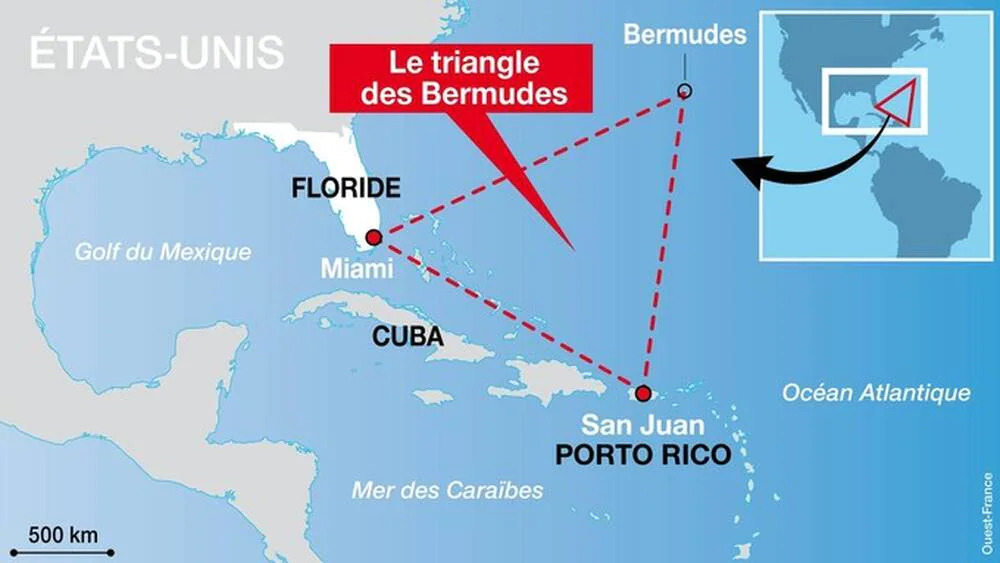
\includegraphics[scale=0.5]{bermudes.jpg}
        \end{center}
    \end{columns}
  \end{frame}

  \begin{frame}{Mort}
    \hypertarget{mort}{}
    \begin{columns}
      \column{0.5\textwidth}
        Tu te trouves au fond du casier de Davy Jones, mais il te prend en pitié.
        Il t'envoie \hyperlink{début}{à ton bâteau}...
      \column{0.5\textwidth}
        \begin{center}
          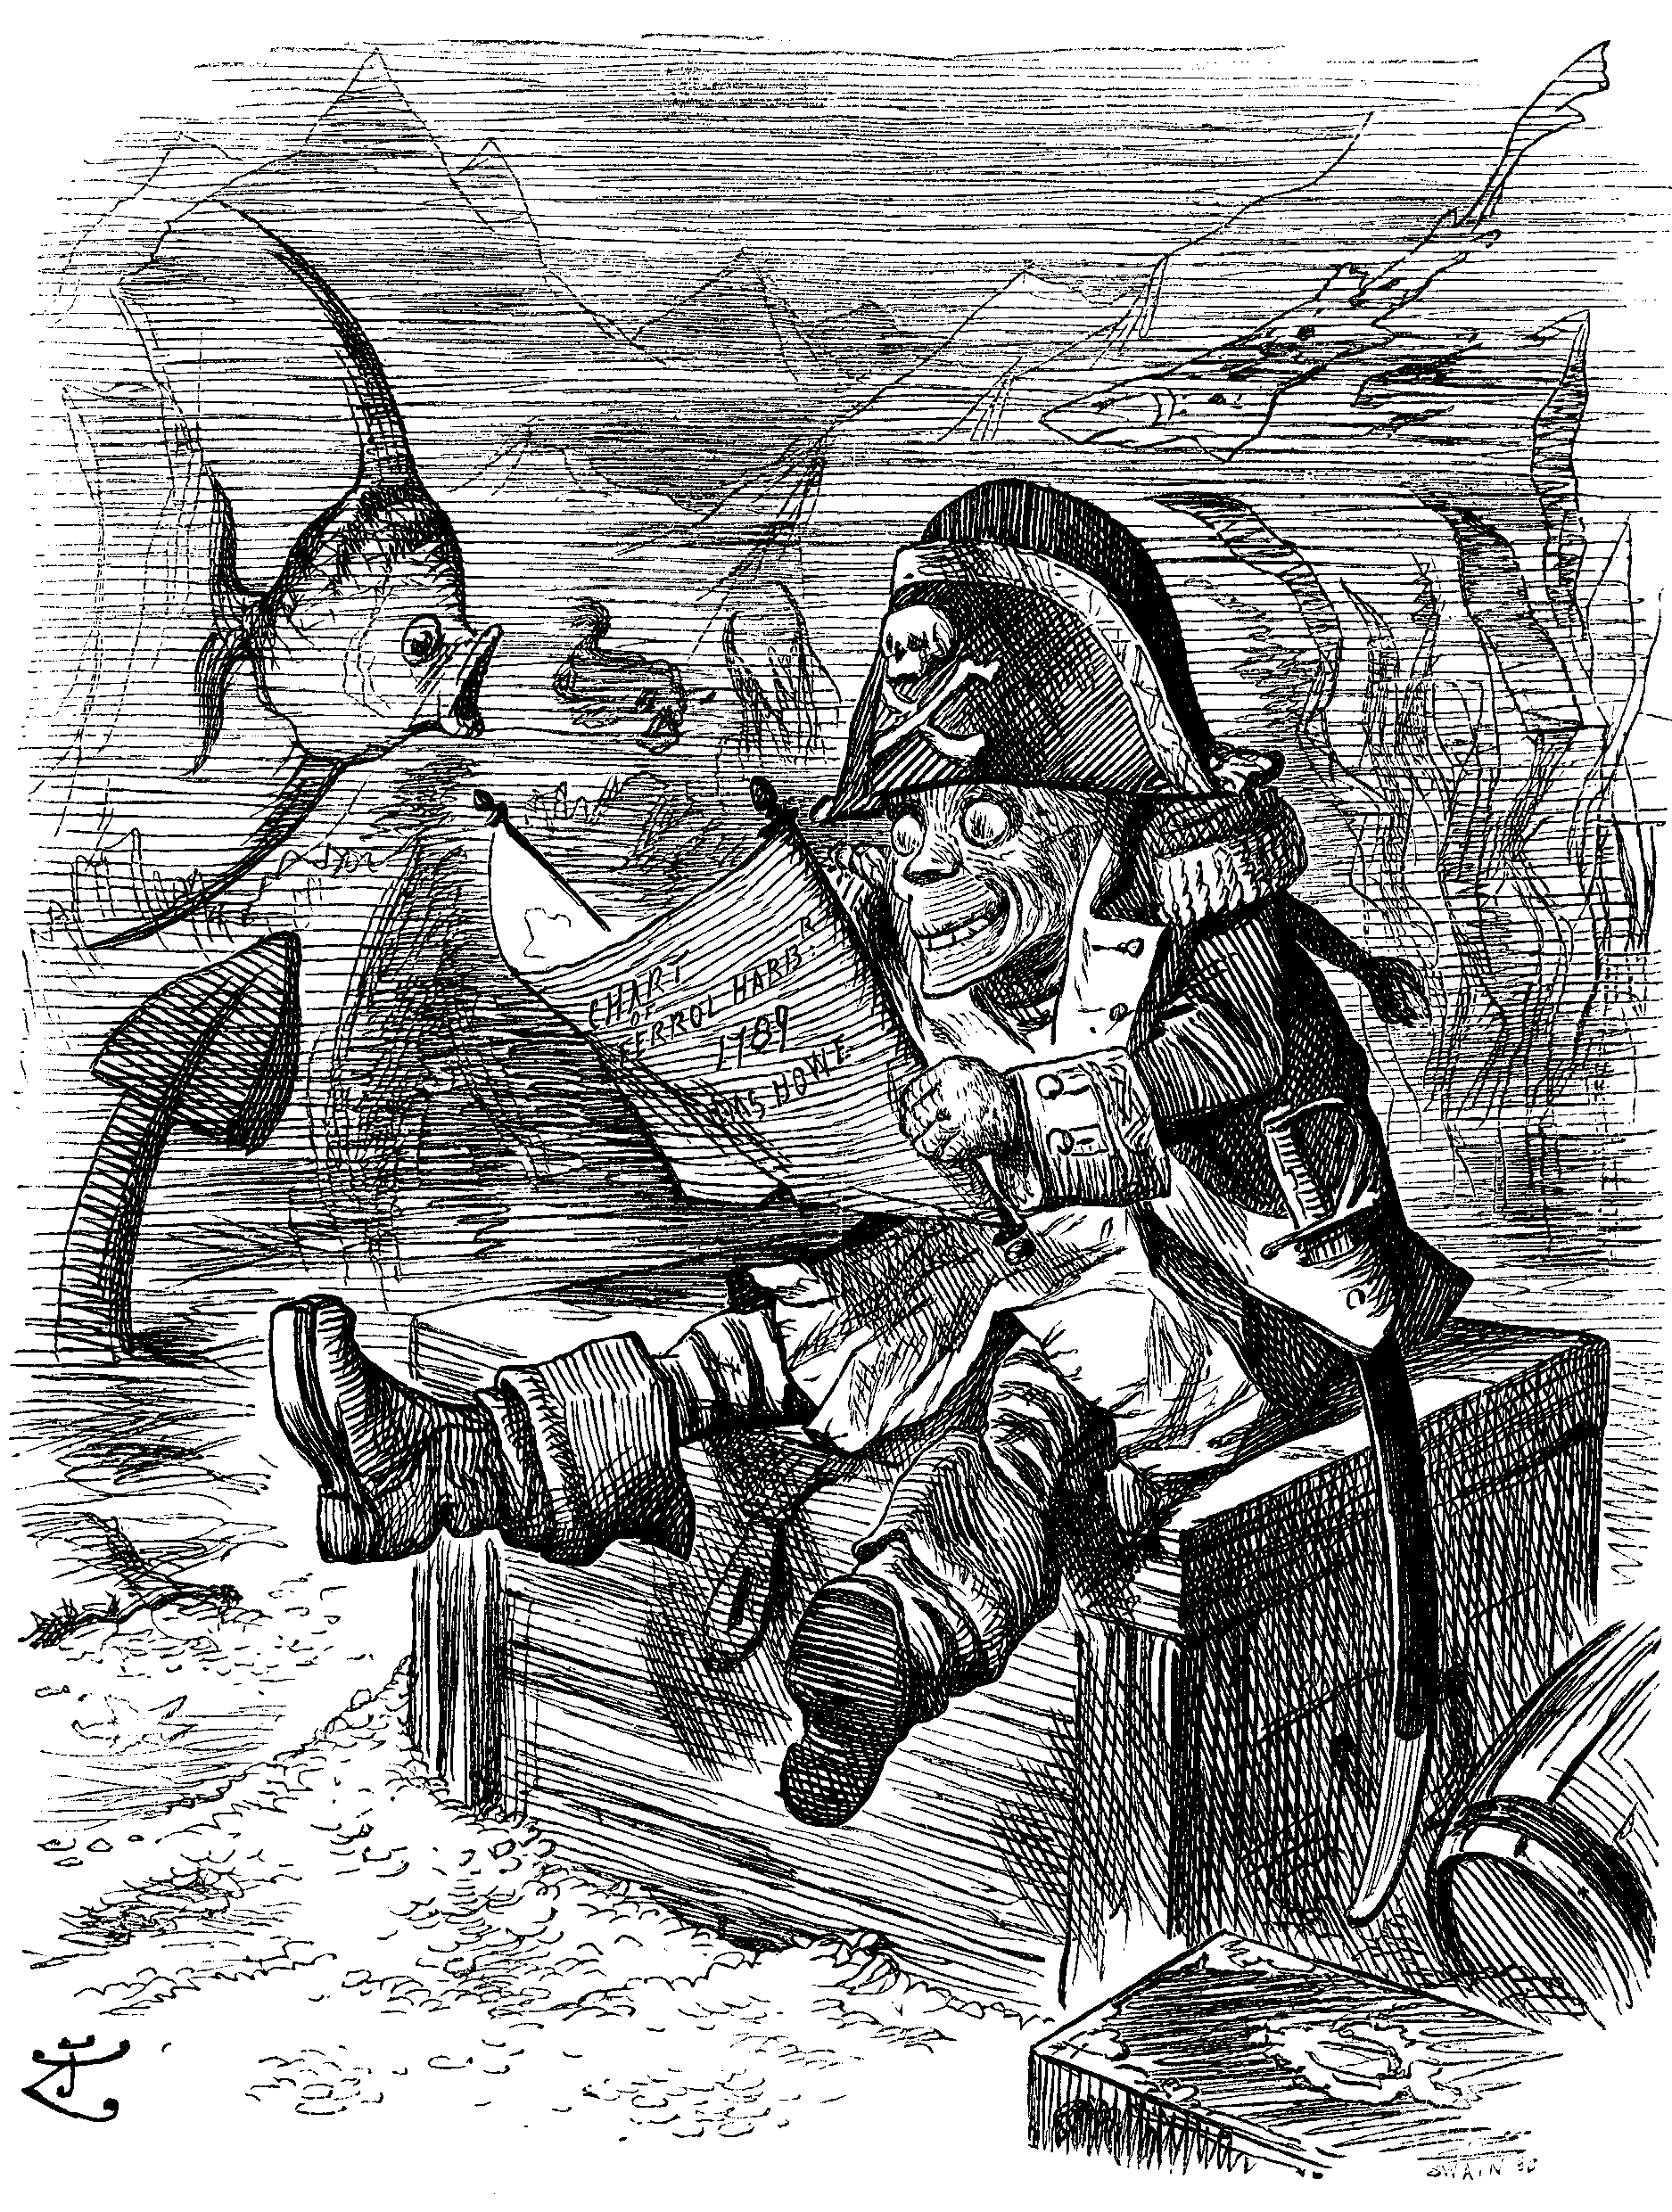
\includegraphics[scale=0.25]{casier.png}
        \end{center}
    \end{columns}
  \end{frame}
\end{document}
